\section{Occupancy-Grid-Mapping}
In dem hiesigen Anwendungsfall sollen metrische Karten verwendet werden, um das Navigationsproblem lösen zu können. Ein passender Kartentyp sind die so genannten Occupancy-Grids, welche die Umgebung als 2- oder 3-dimensionales, diskretes Raster darstellen. Jeder Zelle der Karte wird eine Wahrscheinlichkeit zugeordnet, die wiedergibt, ob die Zelle belegt ist. Durch den stochastischen Charakter des Umgebungsmodells können Ungewissheiten bei der Kartographierung und anschließenden Navigation beachtet werden.

Mathematisch wird die Umgebung als diskrete Menge von binären Zufallsvariablen 
\begin{equation}
M=\{ m_{i} \}
\end{equation}
beschrieben, die entweder den Zustand frei oder belegt annehmen können. Die Aufgabe des Kartographierungsalgorithmus besteht darin, eine Karte zu erstellen, wobei es sich um die a posteriori Wahrscheinlichkeit
\begin{equation}
\condP{M=\text{belegt}}{\vec{z}_{1:t}, \vec{x}_{1:t}}\footnote{Im Folgenden wird die Wahrscheinlichkeit für $M=\text{belegt}$ bzw. $m_i=\text{belegt}$ als $p(M)$ bzw. $p(m_i)$ geschrieben. Die Wahrscheinlichkeiten für freie Zellen werden mit $p(\neg m_i)$ denotiert.}
\end{equation}
handelt. Für jede Zelle soll die Wahrscheinlichkeit, dass diese unter Beachtung aller bisheriger Sensorwerte $\vec{z}_{1:t}$ und aller Zustandswerte $\vec{x}_{1:t}$ belegt ist, ermittelt werden. Um dieses Problem zu lösen, wird als erster Ansatz ein Bayes-Filter für binäre Zufallsvariablen angeführt. Es werden die beiden folgenden Annahmen getroffen: Die Umgebung ist stationär, das heißt keine Objekte werden während der Kartenaufzeichnung verschoben. Somit kann der Algorithmus nicht genutzt werden, um dynamischen Hindernissen auszuweichen. Zweitens wird angenommen, dass die Wahrscheinlichkeiten der einzelnen Zellen unabhängig sind.
\begin{equation}
\condP{M}{\vec{z}_{1:t}, \vec{x}_{1:t}} = \prod_i \condP{m_i}{\vec{z}_{1:t},\vec{x}_{1:t}}\,.
\end{equation}
Dadurch können die a posteriori Wahrscheinlichkeiten der Zellen separat berechnet werden. Allerdings kann diese Annahmen unter realen Umständen kaum verteidigt werden, da Hindernisse für gewöhnlich größer als eine einzelne Kartenzelle sind.

Für die Berechnung der Karte wird das logarithmische Verhältnis
\begin{equation}
l(x) = log\left[ \frac{p(m\idx{i})}{1-p(m\idx{i}} \right] = log\left[ \frac{p(m\idx{i}}{p(\neg m\idx{i}} \right]\,,
\end{equation}
das bei binären Zufallsvariablen  rechentechnische Vorteile mit sich bringt  \cite[S. 94 f]{ProbRob}. Bei der Kartenaufzeichnung soll das logarithmische Verhältnis $l(m\idx{i})_t$ am Zeitpunkt $t$ anhand des vergangen Wertes $l(m\idx{i})_{t-1}$, des Messvektors $\vec{z}_t$ und des Zustandsvektors $\vec{x}_t$ für alle $i$ Zellen der Karte bestimmt werden. Die gesuchte Wahrscheinlichkeit ergibt sich aus
\begin{equation}
\condP{x} = 1 - \frac{1}{1+e^{l(x)_t}}\,.
\end{equation}

Für die Herleitung des Bayes-Filter wird zunächst der Fall betrachtet, dass die Zelle $m_i$ belegt ist. Nach Bayes-Theorem folgt für die a posteriori Wahrscheinlichkeit
\begin{equation}
\label{eq_bayes_filter_1}
\begin{split}
\condP{m_i}{\vec{z}_{1:t}} &= \condP{m_i}{\vec{z}_t, \vec{z}_{1:t-1}} \\
&= \frac{\condP{\vec{z}_t}{m_i, \vec{z}_{1:t-1}}\cdot \condP{m_i}{\vec{z}_{1:t-1}}}{\condP{\vec{z}_t}{\vec{z}_{1:t-1}}} \\
&= \frac{\condP{\vec{z}_t}{m_i}\cdot \condP{m_i}{\vec{z}_{1:t-1}}}{\condP{\vec{z}_t}{\vec{z}_{1:t-1}}}\,.
\end{split}
\end{equation}
Wie Wahrscheinlichkeit $\condP{\vec{z}_t}{m_i}$ wird als Messmodell bezeichnet, da sie angibt, wie wahrscheinlich ein Messwert $\vec{z}_t$ aus einer gegebenen Umgebung $m_i$ folgt. Aus Bayes-Theorem folgt wiederum
\begin{equation}
\condP{\vec{z}_t}{m_i} = \frac{\condP{m_i}{\vec{z}_t}\cdot p(\vec{z}_t}{p(m_i)}
\end{equation}
und die anschließende Substitution in \ref{eq_bayes_filter_1} liefert
\begin{equation}
\condP{m_i}{\vec{z}_{1:t}} = \frac{\condP{m_i}{\vec{z}_t}\cdot p(\vec{z}_t) \cdot \condP{m_i}{\vec{z}_{1:t-1}}}{p(m_i)\cdot \condP{\vec{z}_t}{\vec{z}_{1:t-1}}}\,.
\end{equation}
Analog ergibt sich für das komplementäre Ereignis $\neg m_i$
\begin{equation}
\condP{\neg m_i}{\vec{z}_{1:t}} = \frac{\condP{\neg m_i}{\vec{z}_t}\cdot p(\vec{z}_t) \cdot \condP{\neg m_i}{\vec{z}_{1:t-1}}}{p(\neg m_i)\cdot \condP{\vec{z}_t}{\vec{z}_{1:t-1}}}\,.
\end{equation}
Im nächsten Schritt folgt der Quotient der beiden Verteilungen
\begin{equation}
\begin{split}
\frac{\condP{m_i}{\vec{z}_{1:t}}}{\condP{\neg m_i}{\vec{z}_{1:t}}} &= \frac{\condP{m_i}{\vec{z}_t}\cdot p(\vec{z}_t) \cdot \condP{m_i}{\vec{z}_{1:t-1}} \cdot p(\neg m_i)\cdot \condP{\vec{z}_t}{\vec{z}_{1:t-1}}}{\condP{\neg m_i}{\vec{z}_t}\cdot p(\vec{z}_t) \cdot \condP{\neg m_i}{\vec{z}_{1:t-1}} \cdot p(m_i)\cdot \condP{\vec{z}_t}{\vec{z}_{1:t-1}}} \\
&= \frac{\condP{m_i}{\vec{z}_{1:t-1}}}{\condP{\neg m_i}{\vec{z}_{1:t-1}}} \cdot
\frac{\condP{m_i}{\vec{z}_t}}{\condP{\neg m_i}{\vec{z}_{1:t-1}}}\cdot \frac{p(\neg m_i)}{p(m_i)}\,,
\end{split}
\end{equation}
dessen Logarithmus das gesuchte Verhältnis liefert:
\begin{equation}
\label{eq_bayes_filter_2}
\begin{split}
l(m_i)_t &\equiv \myLog{ \frac{\condP{m_i}{\vec{z}_{1:t}}}{\condP{\neg m_i}{\vec{z}_{1:t}}} }  \\
&= \underbrace{\myLog{ \frac{\condP{m_i}{\vec{z}_{1:t-1}}}{\condP{\neg m_i}{\vec{z}_{1:t-1}}} }}_{= l(m_i)_{t-1}} 
- \underbrace{ \myLog{ \frac{p(\neg m_i)}{p(m_i)} } }_{=l(m_i)_{t=0}\equiv l_0}
 + \myLog{ \frac{\condP{m_i}{\vec{z}_t}}{\condP{\neg m_i}{\vec{z}_{1:t-1}}} }\,.
\end{split}
\end{equation}
Somit setzt sich die gesuchte a posteriori Wahrscheinlichkeit aus drei Summanden zusammen. Bei dem Ersten handelt es sich um die Wahrscheinlichkeit $l(m_i)_{t-1}$ am vorherigen Abtastpunkt. Der Zweite gibt das Verhältnis der a priori Wahrscheinlichkeiten zum Zeitpunkt $t=0$ wider und der letzte Teil ergibt sich aus dem logarithmischen Verhältnis von $\condP{m_i}{\vec{z}_t}$, wobei es sich um ein inverses Messmodell handelt. Die Wahrscheinlichkeit $\condP{m_i}{\vec{z}_t}$ wird von dem Entwickler vorgegeben und basiert auf der Charakteristik der Sensorik.
Als Beispiel dient an dieser Stelle ein rudimentäres Modell für einen Laserscanner. Der Sensor gibt einen Vektor von Distanzmessungen zurück, die jeweils einen Messwinkel $\varphi$ relativ zu dem Roboter zuzuordnen sind. Somit liegt ein Messbereich in Form eines Kegels mit dem Öffnungswinkel $\Delta \varphi$ vor, der durch die gemessenen Distanzen begrenzt wird.
\begin{figure}[!ht]
\centering
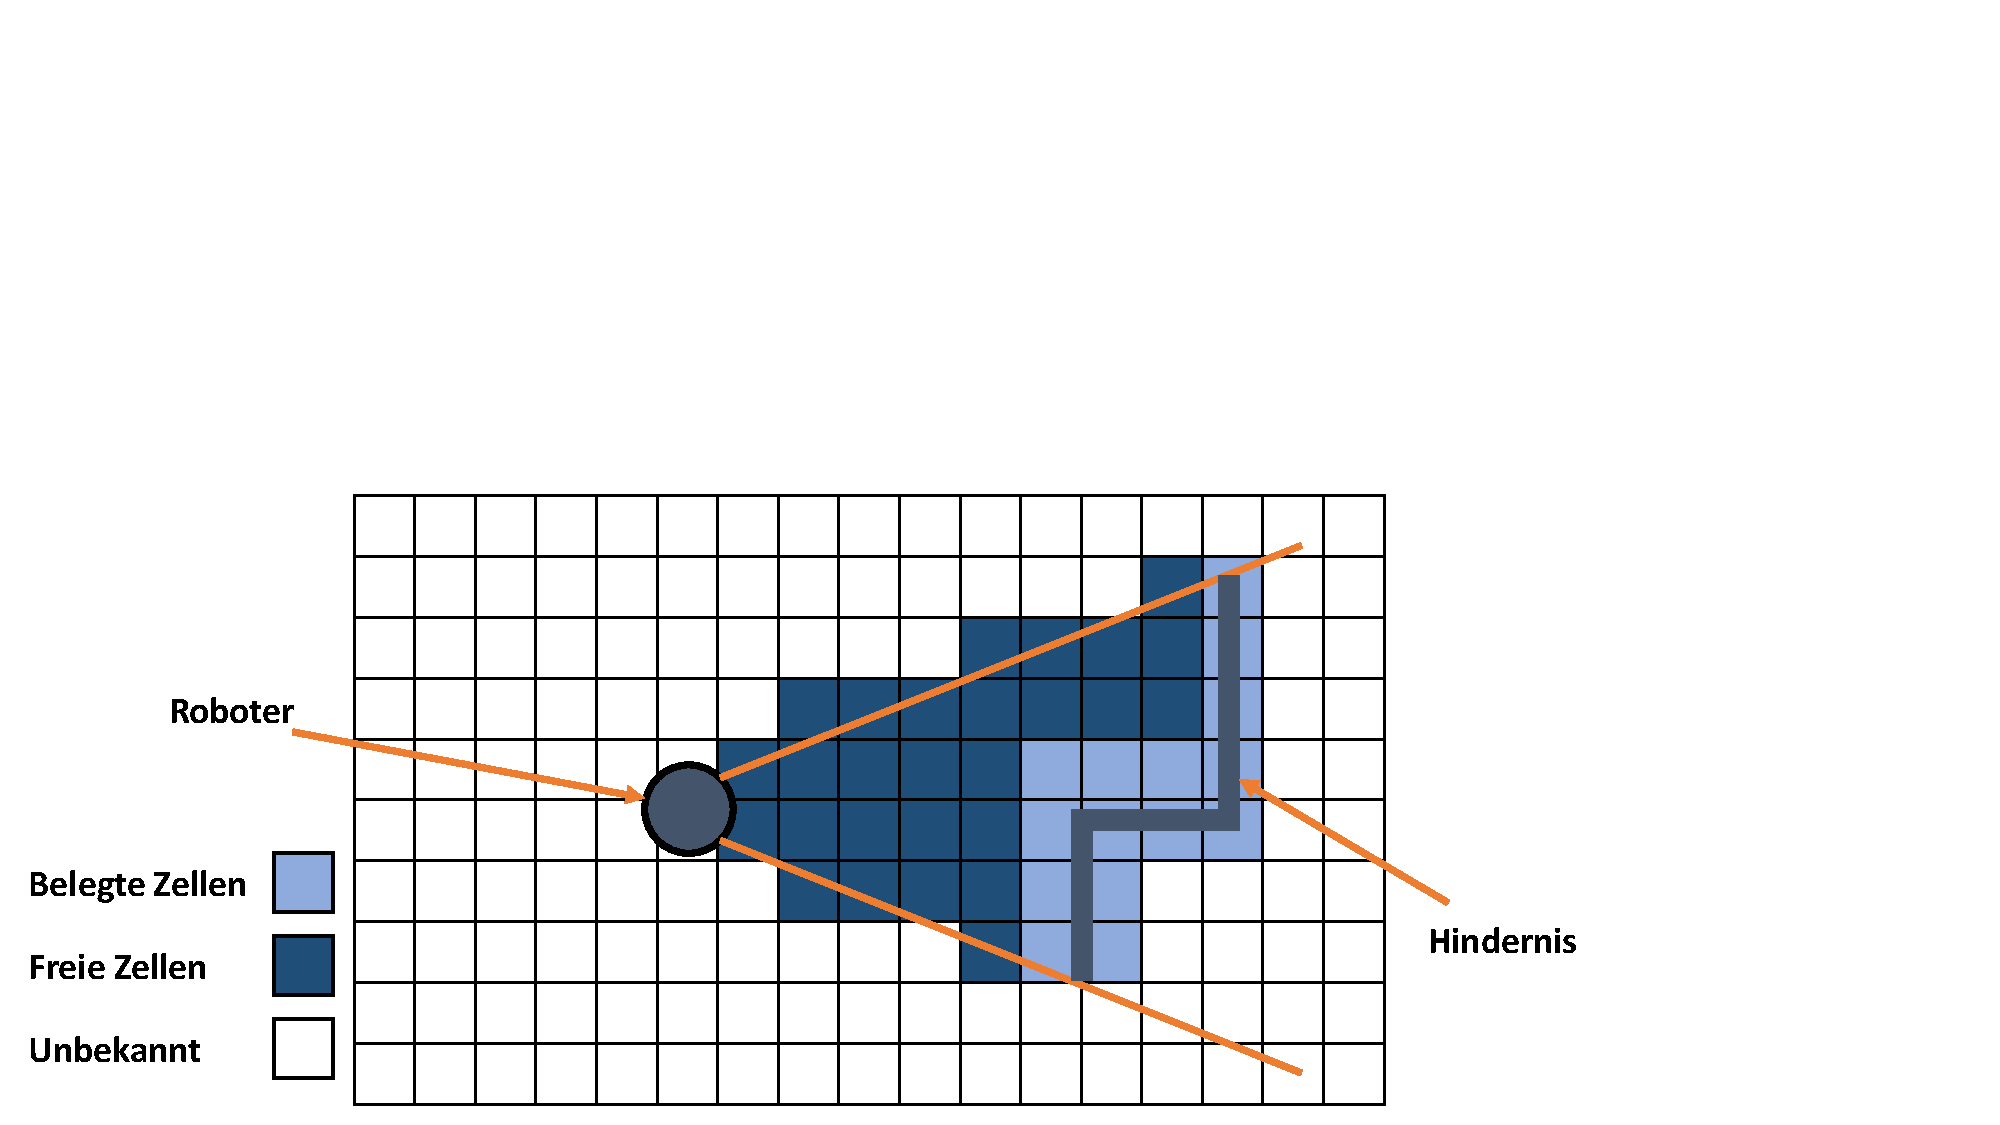
\includegraphics[width=0.7\linewidth, trim={0cm 0cm 7cm 8cm}, clip]{img/Bilder_Karten_InvSensModel_1}
\caption{Schematische Darstellung der Karten und des inversen Messmodells}
\end{figure}
Im inversen Messmodell werden nun drei Fälle unterschieden. Liegt eine Zelle außerhalb des Messkegels, kann keine Aussage über den Zustand der Zelle getroffen werden, weshalb der Wert $l_0$ zurückgegeben wird der in \ref{eq_bayes_filter_2} eingesetzt zu 
\begin{equation}
l(m_i)_t = l(m_i)_{t-1} + l_0 - l_0 = l(m_i)_{t-1}
\end{equation}
führt; die Wahrscheinlichkeit der Zelle bleibt also unverändert. 

In dem Fall, dass die Zelle innerhalb des Messkegels liegt, wird geprüft auf welchem Messstrahl und in welcher Distanz die Zelle sich befindet. Ist der Abstand zwischen der Zelle und der gemessenen Distanz kleiner als ein Toleranzmaß $\alpha$, wird angenommen, dass die Zelle belegt ist und ein entsprechender Wert $l_{\text{occupied}}$ zurückgegeben. Liegt die Zelle mehr als $\alpha$ Einheiten vor der gemessen Distanz, gilt sie als frei und das Modell liefert den Wert $l_{\text{free}}$.